\subsubsection{Y-Axis: Functional Decomposition}

The y-axis scaling focuses on the separation based on the responsibility for an
action which can be determined by the type of data or the type of work performed
for a transaction. While scaling on the x-axis could means "everyone does
everything", scaling on the y-axis specializes the workers splitting the whole
service in small services and assigning each service to a single worker. If we
combine the x-axis with the y-axis, we could have cluster of specialized workers
such that each cluster cover a different service, but workers in the same
cluster do the same job.

With regards to the data, differently from what happens in the x-axis, each
service should have its own non-shared data, thus segmenting it based on what
each service needs to have access to. This allows to size and optimize the
resources based on the transactions demand for each service, and ultimately to
reduce the operational costs.

As done before for the x-axis, we provide an example of an architectural
approach which corresponds on the y-axis.

\paragraph{Microservice architecture}
Recalling the e-commerce example presented above, instead of duplicating the
monolithic application and distribute the load equally between the clones, we
can identify logical components, that is different functional areas of the
application, such as account service, purchase service, product service.

\begin{figure}
	\begin{center}
		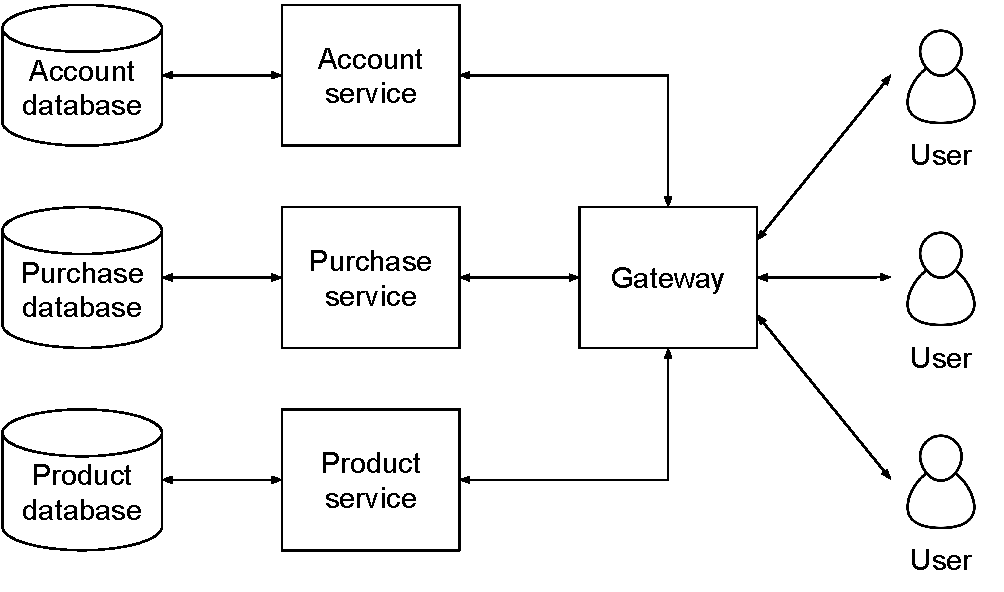
\includegraphics[width=.7\textwidth]{./res/img/microservice-architecture.pdf}
	\end{center}
	\caption{Example of a microservice architecture.}
	\label{fig:microservice-architecture}
\end{figure}

The diagram in \autoref{fig:microservice-architecture} summarises the
microservice architecture resulting from such division. The \emph{user} entity
condenses different client concepts (e.g. browser or mobile applications, bots,
humans, or others), while the \emph{gateway} represents what guide the requests
to the right service. In the case of a browser application, the gateway could
also exists only in it without needing a dedicated back end component, or it
could not exists at all, for example advertising the location of each service
and delegating to the users the responsibility to choose the right service. Each
service has its own non-shared database, which represents a good solution in the
case of perfect isolated services. More often, there could be some logical
relations between data stored in different services making necessary to
implement a mechanism to maintain data consistency.\todo{To complete}